\documentclass[twoside]{article}
\setlength{\oddsidemargin}{-0.5 in}
\setlength{\evensidemargin}{1.5 in}
\setlength{\topmargin}{-0.6 in}
\setlength{\textwidth}{5.5 in}
\setlength{\textheight}{8.5 in}
\setlength{\headsep}{0.5 in}
\setlength{\parindent}{0 in}
\setlength{\parskip}{0.07 in}
\setlength{\marginparwidth}{145pt}

%
% ADD PACKAGES here:
% 12

\usepackage{amsmath,
            amsfonts,
            amssymb,
            graphicx,
            mathtools,
            flexisym,
            marginnote,
            hyperref,
            titlesec}

\usepackage[english]{babel}
\usepackage[utf8]{inputenc}
\usepackage[shortlabels]{enumitem}

\graphicspath{ {images/} }

\hypersetup{
    colorlinks=true,
    linkcolor=blue,
    filecolor=magenta,      
    urlcolor=blue,
}

\titlespacing\section{0pt}{12pt plus 4pt minus 2pt}{0pt plus 2pt minus 2pt}
\titlespacing\subsection{0pt}{12pt plus 4pt minus 2pt}{0pt plus 2pt minus 2pt}

%
% The following commands set up the lecnum (lecture number)
% counter and make various numbering schemes work relative
% to the lecture number.
%
\newcounter{lecnum}
\renewcommand{\thepage}{\thelecnum-\arabic{page}}
\renewcommand{\thesection}{\thelecnum.\arabic{section}}
\renewcommand{\theequation}{\thelecnum.\arabic{equation}}
\renewcommand{\thefigure}{\thelecnum.\arabic{figure}}
\renewcommand{\thetable}{\thelecnum.\arabic{table}}

\newcommand{\aosv}{1044414: Advanced Operating Systems and Virtualization}
\newcommand{\wir}{1038137: Web Information Retrieval}
\newcommand{\va}{1052057: Visual Analytics}
\newcommand{\advprog}{1044416: Advanced Programming}
\newcommand{\dchpc}{1044399: Data Centers and High Perf. Computing}

\newcommand{\qu}[1]{\marginnote{\textcolor{cyan}{#1}}}


%
% The following macro is used to generate the header.
%
\newcommand{\lecture}[4]{
   \pagestyle{myheadings}
   \thispagestyle{plain}
   \newpage
   \setcounter{lecnum}{#4}
   \setcounter{page}{1}
   \noindent
   \begin{center}
   \framebox{
      \vbox{\vspace{2mm}
    \hbox to 7.4in { {\bf #1
    \hfill Spring 2018} }
       \vspace{4mm}
       \hbox to 7.4in { {\Large \hfill Lecture #4: #2  \hfill} }
       \vspace{2mm}
       \hbox to 7.4in { {\it Lecturer: #3 \hfill Scribe: Anxhelo Xhebraj} }
      \vspace{2mm}}
   }
   \end{center}
   \markboth{Lecture #4: #2}{Lecture #4: #2}

   \iffalse
   {\bf Note}: {\it LaTeX template courtesy of UC Berkeley EECS dept.}

   {\bf Disclaimer}: {\it These notes have not been subjected to the
   usual scrutiny reserved for formal publications.  They may be distributed
   outside this class only with the permission of the Instructor.}
   \vspace*{4mm}
   \fi
}
%
% Convention for citations is authors' initials followed by the year.
% For example, to cite a paper by Leighton and Maggs you would type
% \cite{LM89}, and to cite a paper by Strassen you would type \cite{S69}.
% (To avoid bibliography problems, for now we redefine the \cite command.)
% Also commands that create a suitable format for the reference list.
\iffalse
\renewcommand{\cite}[1]{[#1]}
\def\beginrefs{\begin{list}%
        {[\arabic{equation}]}{\usecounter{equation}
         \setlength{\leftmargin}{2.0truecm}\setlength{\labelsep}{0.4truecm}%
         \setlength{\labelwidth}{1.6truecm}}}
\def\endrefs{\end{list}}
\def\bibentry#1{\item[\hbox{[#1]}]}
\fi

%Use this command for a figure; it puts a figure in wherever you want it.
%usage: \fig{NUMBER}{SPACE-IN-INCHES}{CAPTION}
\newcommand{\fig}[3]{
            \vspace{#2}
            \begin{center}
            Figure \thelecnum.#1:~#3
            \end{center}
    }
% Use these for theorems, lemmas, proofs, etc.
\newtheorem{theorem}{Theorem}[lecnum]
\newtheorem{lemma}[theorem]{Lemma}
\newtheorem{proposition}[theorem]{Proposition}
\newtheorem{claim}[theorem]{Claim}
\newtheorem{corollary}[theorem]{Corollary}
\newtheorem{definition}[theorem]{Definition}
\newenvironment{proof}{{\bf Proof:}}{\hfill\rule{2mm}{2mm}}

% **** IF YOU WANT TO DEFINE ADDITIONAL MACROS FOR YOURSELF, PUT THEM HERE:

\newcommand\E{\mathbb{E}}

\begin{document}

\nocite{*}

%FILL IN THE RIGHT INFO.
%\lecture{**LECTURE-NUMBER**}{**DATE**}{**LECTURER**}{**SCRIBE**}

\lecture{\aosv}{March 6}{Alessandro Pellegrini}{2}

%\footnotetext{These notes are partially based on those of Nigel Mansell.}

% **** YOUR NOTES GO HERE:

\iffalse

\section{Stage 1 Bootloader}
After disabling the interrupts and having initialized all the segments registers to 0 the A20 line is enabled and the switch to 32 bit protected mode is performed. Finally a stack is setup and the Stage 2 Bootloader is loaded (if BIOS mode and not UEFI).

\fi

\section{A20 Line}

\subsection{Story}
The \marginnote{\textsc{Memory Wrap-Around}} original 8086 processor featured a 20-bit address bus capable of addressing 1MB of memory. However, the odd segmentation mechanism, theoretically, allowed addressing slightly more than just 1MB. Indeed all the \textit{logical} addresses ranging from \texttt{F800:8000} (or equivalently \texttt{FFFF:0010}) to \texttt{FFFF:FFFF} and their \textit{linear} equivalent \texttt{0x100000} and \texttt{0x10FFEF} did not have a corresponding \textit{physical} address.

The workaround for this issue was Memory Wrap-Around: "wrap" that portion of memory making those addresses point to the lower portion of memory by dropping bit 20  (indexing bits from 0 from the least significant). This means that the physical addresses shown above would be mapped to \texttt{0x00000} and \texttt{0x0FFEF}.

Such workaround was then used heavily by many programmers to improve performances of their programs. For example it was used by DOS programmers in order to use the same segment for accessing both program data placed in the higher part of the memory and I/O data that was placed in the lower end. 

Introducing \marginnote{\textsc{A20 Line Fix}} the Intel 80286 the addressable memory was increased to 16 MB in protected mode, however the new CPU was supposed to be able to run in real mode all programs developed for the 8086 so that it could run OSes and programs that were not written for protected mode. This produced a bug in the IBM PC AT computer since logical address \texttt{F800:8000} accessed the physical address \texttt{0x100000} instead of wrapping around and access \texttt{0x00000}. The issue was solved by ANDING the CPU A20 (address line 20) with an output of the keyboard controller (KBC).

Disconnecting just A20 and not also A21, A22, A23 was enough since real mode software cared only about the area slightly above 1MB.

\subsection{Enabling A20 Line via keyboard controller}
A20 Line can be enabled through various methods but the classical one is through the keyboard controller which at the time was just a single chip (8042) today known as PS/2 Controller.

The PS/2 Controller uses 2 IO ports: port \texttt{0x60} for reading/writing data from/to the controller and port \texttt{0x64} for reading/writing the status/command register of the controller. Bit 1 of the status register tells the Input buffer status of the controller: 0 if empty, 1 if full. It must be clear before attempting to write some data to port \texttt{0x60} or \texttt{0x64} therefore we must use the busy waiting scheme to communicate with the controller.

By writing in the command register the value \texttt{0xD1} we ask the controller to write the next byte (that will be sent to it in the data register) to the Controller Output Port. \texttt{0xDF} is the code for enabling the A20 line and \texttt{0xDD} for disabling it. 

Follows the code for enabling A20.

\begin{verbatim}
    ...
    call wait_for_8042    ; busywait to be able to write the command
    movb $0xd1, %al
    outb %al, $0x64       ; ask to write
    call wait_for_8042
    movb $0xdf, %al
    outb %al, $0x60       ; enable A20
    call wait_for_8042
    ...
  
  wait_for_8042:          ; busy waiting routine
    inb %al, $0x64
    testb $2, %al         ; check if can write (Bit 1 has value 1 if full)
    jnz wait_for_8042
    ret
\end{verbatim}

\section{Protected Mode Overview}

Protected mode gets its name from the privilege protection \marginnote{
  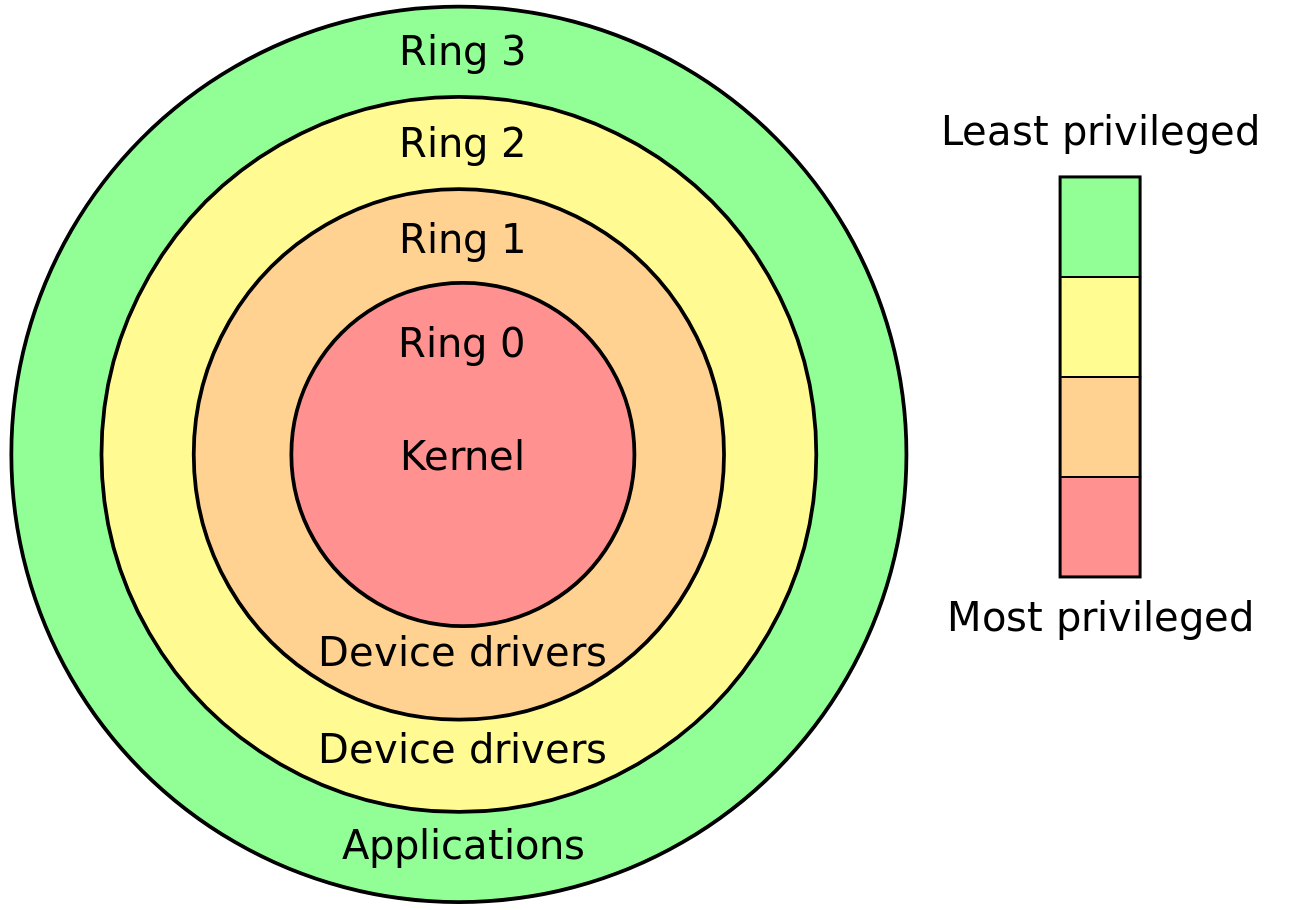
\includegraphics[width= 0.35 \textwidth]{privlevel.png}
  \fig{1}{0 pt}{Intel CPU privilege levels}
}[-1 cm]
mechanisms introduced in the Intel 386 processor to restrict what user-level programs can do employing \textbf{Privilege Levels}. There are four privilege levels, numbered 0 (most privileged) to 3 (least privileged), and three main resources being protected: memory, I/O ports, and the ability to execute certain machine instructions.
Protected mode was then extended by adding paging. Both paging and protected mode must be enabled on startup.
At any given time, an x86 CPU is running in a specific privilege level, which determines what code can and cannot do. These privilege levels are often described as \textbf{Protection Rings}, with the innermost ring corresponding to highest privilege. Most modern x86 kernels use only two privilege levels, 0 and 3. Ring 1 has been used in hypervisor systems.

To manage these kind of security mechanisms a new set of registers, namely Control Registers, were introduced. About 15 machine instructions, out of dozens, are restricted by the CPU to ring zero. In protected mode \textbf{only privilege level 0} code can read or load the Control Registers. In user space CS is not writable.

The \marginnote{\textsc{Control Register 0}} most important Control Register is CR0 which contains system control flags that control operating mode and states of the processor:
\begin{description}
  \itemsep0em
  \item [PG Paging (bit 31):] Enables paging when set; disables paging when clear. When paging is
  disabled, all linear addresses are treated as physical addresses. The PG flag has no effect if the PE flag (bit
  0 of register CR0) is not also set; setting the PG flag when the PE flag is clear causes a general-protection
  exception (\#GP)
  \item [CD Cache Disable (bit 30):] together with NW, when set, fully disable caches
  \item [NW Not Write-through (bit 29)]
  \item [NE Numeric Error (bit 5):] enables the reporting of x87 FPU errors
  \item [PE Protection Enable (bit 0):] Enables protected mode when set; enables real-address mode when clear. This flag does not enable paging directly. It only enables segment-level protection. To enable paging, both the PE and PG flags must be set \marginnote{The OS may sometimes set PE to 0 to write big chunks of memory to improve performance and then reset it}[-36 pt]
\end{description}

By switching to protected mode we get that all the instructions that the processor will start executing will be interpreted as 32-bit from now on instead of 16-bit. By this fact two problems might arise: the \texttt{CS} register contains information that had some meaning in real mode but not the same in protected mode and the CPU prefetches the instructions it has to execute in an \textbf{Instruction Queue} and interprets it as an \textit{instruction stream} to be more performant but in this case we are switching from 16 bit to 32 bit. In order to make the CPU to work properly we must perform a far \texttt{jmp} or \texttt{call} instruction to \textit{serialize} the CPU, i.e. flush the Instruction Queue and start reading 32-bit instructions and "re-initialise" the code segment. Afterwards we must also reset Segment Registers since they had the content of 16-bit data/operations. \marginnote{\cite{intel} Ch. 9, Sec. 9.9}[-36 pt]

\section{Memory Translation in Protected Mode}

Before entering protected mode, auxiliary data structures must be setup in order for the system to work properly.

One of the main differences between the two modes of operation (real and protected) are the translation from logical addresses to physical ones. In 32-bit protected mode, a segment selector is no longer a raw number, but instead it contains an index pointing to a 64 bit entry in a table of \textbf{segment descriptors}.

The segment descriptors are stored in two tables: the \textbf{Global Descriptor Table} (GDT) and the \textbf{Local Descriptor Table} (LDT). Each CPU (or core) in a computer contains a register called \textbf{GDTR} which stores the linear memory address of the first byte in the GDT (analogously a register for the LDT). \marginnote{There is one GDT per CPU in multi core systems while there can be many LDTs. LDTs are not really used anymore}[-36 pt]

To choose a segment, you must load a segment register with a \textbf{segment selector} in the following format: \marginnote{RPL field is called CPL in the case of Code Segment Selector and Stack Segment Selector meaning Current Privilege Level}[2 cm]

\begin{center}
  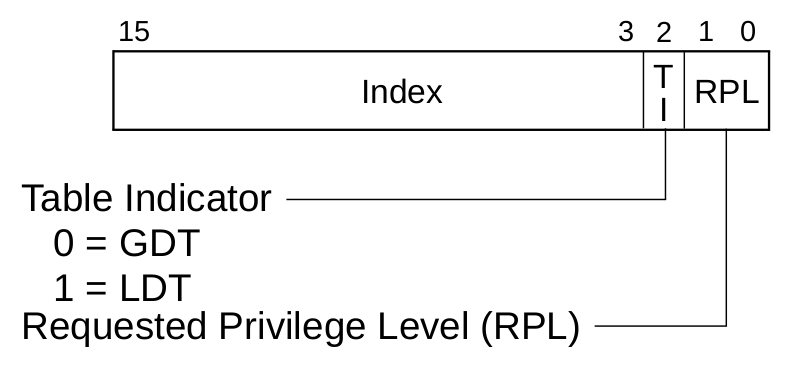
\includegraphics[width=0.5\textwidth]{segsel.png}
  \fig{2}{0 pt}{Segment Selector Format \cite{intel}}
\end{center}

The \textbf{Index} part of the selector identifies which Segment Descriptor (and therefore Segment) we are interested in\marginnote{The size of the table can be at most $2^{13}$ descriptor entries}[-12 pt]. The \textbf{Requested Privilege Level} will be covered later.

Each Segment Descriptor has the following format

\begin{center}
  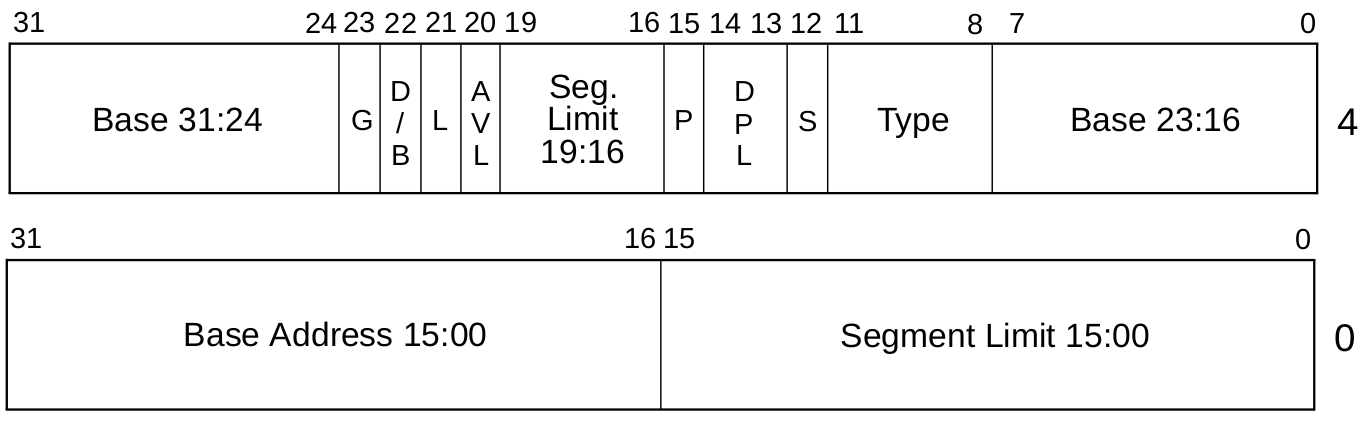
\includegraphics[width=0.8\textwidth]{segdesc.png}
  \fig{3}{0 pt}{Segment Descriptor Entry \cite{intel}}
\end{center}

\begin{description}
  \item [S (descriptor type flag)] Specifies \marginnote{The first descriptor entry in the GDT is not used and its value is all 0s (\cite{intel} pp. 103)} whether the segment descriptor is for a \textbf{system} segment (S flag is clear) or a \textbf{code} or \textbf{data} segment (S flag is set)
  \item [Base] Defines the location of byte 0 of the segment within the 4-GByte linear address space
  \item [Segment Limit] Specifies the size of the segment. The processor puts together the two segment limit fields to form a 20-bit value. The processor interprets the segment limit in one of two ways, depending on the setting of the G (granularity) flag
  \item [G] Determines the scaling of the segment limit field. When the granularity flag is clear, the segment limit is interpreted in byte units; when flag is set, the segment limit is interpreted in 4-KByte units.
  \item [DPL] Is the \textbf{Descriptor Privilege Level}; it is a number from 0 (most privileged, kernel mode) to 3 (least privileged, user mode) that controls access to the segment as will be shown.
\end{description}

\begin{center}
  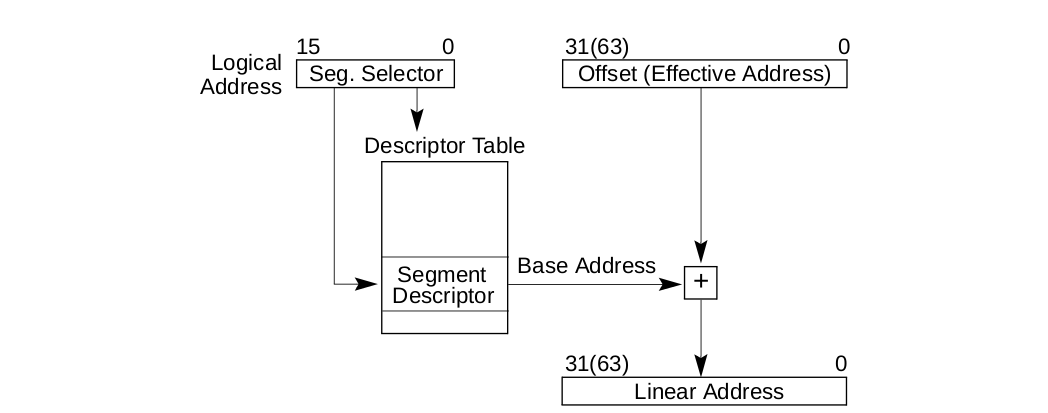
\includegraphics[width=0.8\textwidth]{logadd.png}
  \fig{4}{0 pt}{Logical to Linear Address \cite{intel}}
\end{center}

So how is addressing resolved now? Let's look at an example in case of the instruction \\ \texttt{jmp 0xDEADBEEF}

\begin{enumerate}
  \item The processor looks at the value in the Code Segment (\texttt{CS}) Register and checks \texttt{TI} to know whether to look in the Global or Local table (Suppose Global in the next steps).
  \item Computes the \textit{linear} address \texttt{Index * 8 + GDTR} (8 Bytes is the size of a Segment Descriptor Entry) and fetches the \texttt{Base} of that Segment Descriptor
  \item Computes the linear address that is \texttt{Base + 0xDEADBEEF}
\end{enumerate}

Are all those steps \marginnote{\textsc{Flat Model}} really necessary? No. Segmentation has no real advantage in modern x86 kernels due to the fact that all the memory available is addressable through regular registers but since it is not possible to disable the Segmentation Unit, Intel solved the issue by introducing the \textbf{Flat Model} which means to create just two descriptors for each of the two privilege levels 0 and 3, one for the code segment and one for the data segment both having \texttt{Base} 0 and having as \texttt{Limit} the maximum memory available in 32-bit (4GB). This produces a memory access model as if it was linear.

Since \marginnote{The hidden part is the one used by the processor for fetching the first instruction after a reset} a full communication to memory would be too costly in terms of performance a segment register cache has been introduced also known as "descriptor cache" or "shadow register". The hidden part of the register \textit{is not} invalidated when the entry pointed by that selector changes producing some interesting results. Such |  "unattended" feature allowed programmers to address more than 1MB in the so called "Unreal Mode".

\section{x86 Protection}

Due to restricted access to memory and I/O ports, user mode can do almost nothing to the outside world without calling on the kernel. It can't open files, send network packets, print to the screen, or allocate memory. User processes run in a severely limited sandbox set up by the gods of ring zero. That's why it's impossible, by design, for a process to leak memory beyond its existence or leave open files after it exits. All of the data structures that control such things - memory, open files, etc - cannot be touched directly by user code; once a process finishes, the sandbox is torn down by the kernel.

Keep in mind that the CPU privilege level has nothing to do with operating system users. Whether you're root, Administrator, guest, or a regular user, it does not matter. All user code runs in ring 3 and all kernel code runs in ring 0, regardless of the OS user on whose behalf the code operates. Sometimes certain kernel tasks can be pushed to user mode, for example user-mode device drivers.

The whole protection of the system is based on DPL (Descriptor Privilege Level), RPL (Requested Privilege Level), CPL (Current Privilege Level). The first two are stored respectively in the Segment Descriptor and in the Data Segment Selector while the third one is present in Code Segment Selector stored in the Code Segment Register.

The processor uses privilege levels to prevent a program or task operating at a lesser privilege level from accessing a segment with a greater privilege, except under controlled situations.

Normally, the CPL is equal to the privilege level of the code segment from which instructions are being fetched. The processor changes the CPL when program control is transferred to a code segment with a different privilege level.

The CPU protects memory at two crucial points: when a segment selector is loaded and when a page of memory is accessed with a linear address. Protection thus mirrors memory address translation where both segmentation and paging are involved.

\begin{center}
  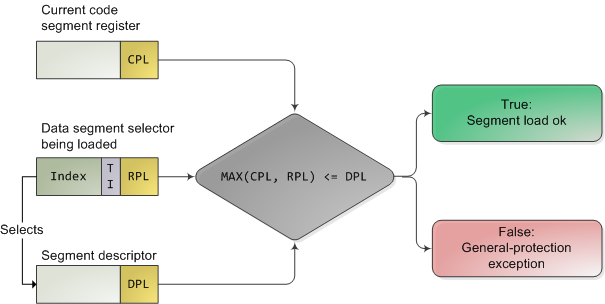
\includegraphics[width=0.8\textwidth]{segproc.png}
  \fig{5}{0 pt}{Segment Privilege Check \cite{duarte_2017}}
\end{center}

In truth, segment protection scarcely matters because modern kernels use a flat address space where the user-mode segments can reach the entire linear address space. Useful memory protection is done in the paging unit when a linear address is converted into a physical address.

\section{Switching between privilege levels}

Another data structure must be setup before entering Protected Mode: the \textbf{Interrupt Descriptor Table}. Such data structure is then used by the OS to handle interrupts and switch between privilege levels.

\subsection{Interrupt Descriptor Table}

In real mode interrupts are handled through the \textbf{Interrupt Vector Table (IVT)} which is a table, typically located at \texttt{0000:000H}, that specifies the addresses of all the 256 \textit{Interrupt Service Routine}. In the case of protected mode the table can be placed anywhere as long the IDTR is set to the right address pointing to its start. The \textbf{IDT} stores a collection of system type segment descriptors (S field cleared in the segment descriptor entry) called \textbf{Gate Descriptors}.

System type descriptors fall in two categories: system-segment descriptors and gate descriptors. System-segment descriptors point to system segments (LDT and \textbf{Task-state segment} segments). Gate descriptors are in themselves "gates", which hold pointers to procedure entry points in code segments (\textbf{call}, \textbf{interrupt}, and \textbf{trap} gates) or which hold segment selectors for TSS’s (\textbf{task} gates). \marginnote{Interrupts are asynchronous events not related to the CPU execution flow while Traps (or exceptions) are synchronous. Traps are the historyical way to demand access to kernel mode}[-36 pt] Call gates provide a kernel entry point that can be used with ordinary call and jmp instructions, but they aren't used much so we'll ignore them. Task gates aren't so hot either (in Linux, they are only used in double faults, which are caused by either kernel or hardware problems). 

Gate descriptors in the IDT can be \textbf{interrupt}, \textbf{trap}, or \textbf{task gate} descriptors.

Each interrupt is assigned a number \textbf{between 0 and 255} called a vector, which the processor uses as an index into the IDT when figuring out which gate descriptor to use when handling the interrupt.

\subsection{Privilege level switch}

To access an interrupt or exception handler, the processor first receives an interrupt vector from internal hardware, an external interrupt controller, or
from software. The interrupt vector provides an index into the IDT. If the selected gate descriptor is an interrupt gate or a trap gate, the associated handler procedure is accessed in a manner similar to calling a procedure through a call gate. If the descriptor is a task gate, the handler is accessed through a task switch.

\begin{center}
  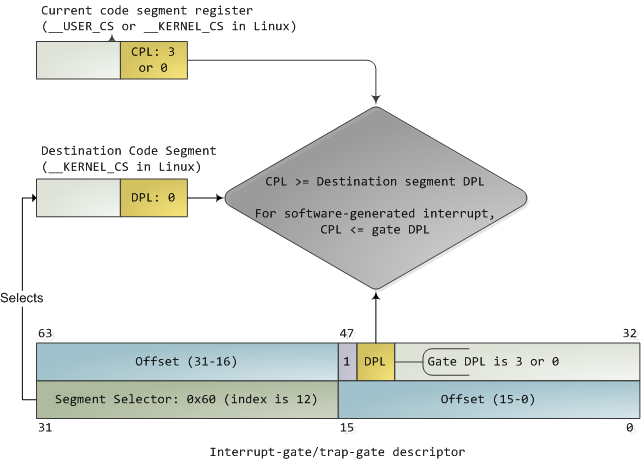
\includegraphics[width=0.8\textwidth]{intdescprv.png}
  \fig{6}{0 pt}{Privilege Management on Interrupt/Exception \cite{duarte_2017}}
\end{center}

An interrupt can never transfer control from a more-privileged to a less-privileged ring. Privilege must either stay the same (when the kernel itself is interrupted) or be elevated (when user-mode code is interrupted) to make sure that the interrupts are handled only by Privilege Level 0 code. In either case, the resulting CPL will be equal to the DPL of the destination code segment; if the CPL changes, a stack switch also occurs. If an interrupt is triggered by code via an instruction like \texttt{int n}, one more check takes place: the gate DPL must be at the same or lower privilege as the CPL. This prevents user code from triggering random interrupts placed in more privileged code segments. If these checks fail a general-protection exception happens. All Linux interrupt handlers end up running in ring zero. 

\textcolor{red}{comm} \iffalse TLS thread local storage, used to set the fs and gs segments, used to describe in a multithreaded application where each thread finds its local copy of ?.} \fi


\subsection{TSS Task State Segment}
The Task State Segment (TSS) is a special data structure for x86 processors which holds information about a task. The TSS is primarily suited for hardware multitasking, where each individual process has its own TSS.

The task register holds the 16-bit segment selector, base address, segment limit, and descriptor attributes for the TSS of the current task which can be placed anywhere in memory.

\marginpar{
  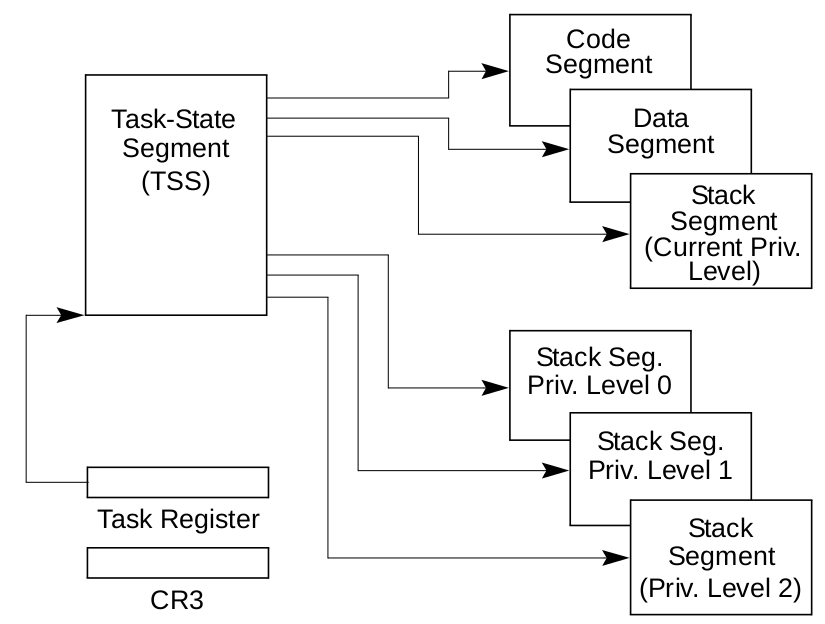
\includegraphics[width=0.4\textwidth]{taskstut.png}
  \fig{7}{0 pt}{Task Management \cite{intel}}
}

The task's current execution space is defined by the segment selectors in the segment
registers (CS, DS, SS, ES, FS, and GS).

Although a TSS could be created for each task running on the computer, Linux kernel only creates one TSS for each CPU as required by the processor architecture and uses them for all tasks. This approach was selected as it provides easier portability to other architectures (for example, the AMD64 architecture does not support hardware task switches), and improved performance and flexibility. Linux only uses the I/O port permission bitmap and inner stack features of the TSS; the other features are only needed for hardware task switches, which the Linux kernel does not use.

\newpage

\marginnote{
  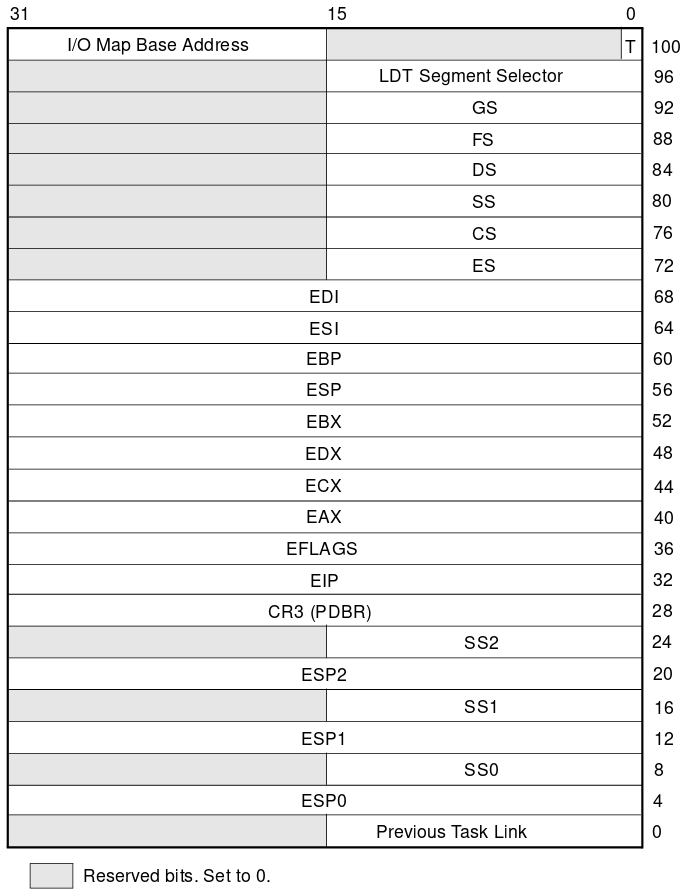
\includegraphics[width=0.4\textwidth]{tss.png}
  \fig{8}{0 pt}{TSS \cite{intel}}
}[2cm]

\begin{center}
  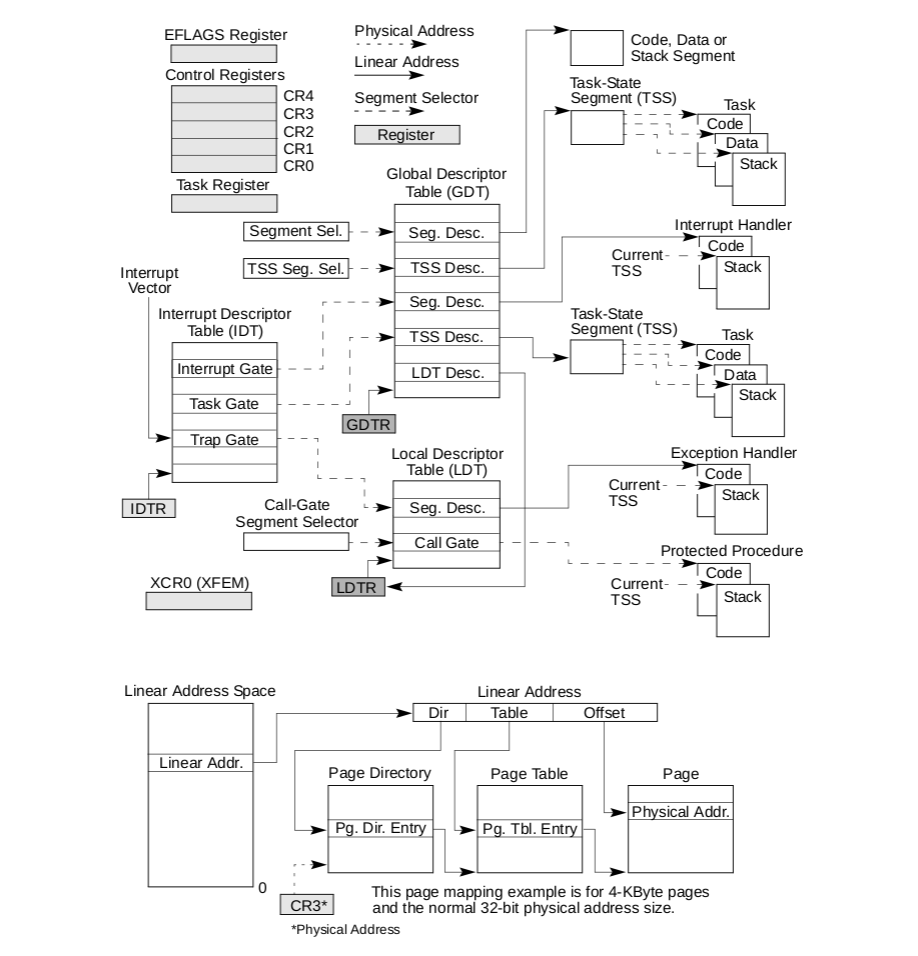
\includegraphics[width=\textwidth]{sysds.png}
  \fig{9}{0 pt}{Data Structures Overview \cite{intel}}
\end{center}


\newpage
\bibliography{Lec2}
\bibliographystyle{plainnat}
\end{document}